\documentclass[11pt,a4paper]{article}

\usepackage[
    a4paper,
    left=15mm,
    right=15mm,
    top=30mm,
    bottom=25mm,
    headheight=25mm
]{geometry}
\usepackage{graphicx}
\usepackage{polski}
\usepackage[utf8]{inputenc}
\usepackage{enumerate}
\usepackage{comment}
\usepackage{fancyhdr}
\usepackage{hyperref}
\usepackage{indentfirst}
\usepackage{multirow}
\usepackage{multicol}
\usepackage{float}
\usepackage{amsmath}
\usepackage{amssymb}
\usepackage{wrapfig}
\usepackage{layout}
\usepackage{textcomp}
\usepackage[center]{caption}
\usepackage{subcaption}
\usepackage{siunitx}
\usepackage[mathscr]{euscript}
\usepackage{xcolor,colortbl}
\usepackage{setspace}
\usepackage{algorithm}
\usepackage[rightComments=false]{algpseudocodex}
\usepackage{listings}
\usepackage{amsthm}
\usepackage{needspace}

% no lone first/last lines of a paragraph on a page
\widowpenalty=10000
\clubpenalty=10000
\displaywidowpenalty=10000

\sisetup{output-exponent-marker=\ensuremath{\mathrm{e}}, output-decimal-marker={,}}
\algrenewcommand\algorithmicprocedure{\textbf{Procedura}}
\algrenewcommand\algorithmicfor{\textbf{Dla}}
\algrenewcommand\algorithmicdo{\textbf{powtarzaj}}
\algrenewcommand\algorithmicwhile{\textbf{Dopóki}}
\algrenewcommand\algorithmicloop{\textbf{Powtarzaj}}
\algrenewcommand\algorithmicif{\textbf{Jeżeli}}
\algrenewcommand\algorithmicelse{\textbf{Inaczej}}
\algrenewcommand\algorithmicthen{\textbf{wykonaj}}
\algrenewcommand\algorithmicend{\textbf{Koniec}}
\algrenewcommand\algorithmicreturn{\textbf{zwróć}}

\newenvironment{algorytm}[1][htb]
  {\par\bigskip\floatname{algorithm}{}\renewcommand{\thealgorithm}{}
   \begin{algorithm}[#1]%
  }{\end{algorithm}\par\bigskip}

\renewcommand{\baselinestretch}{1.18}
\renewcommand\thesubfigure{\roman{subfigure}}

\renewcommand\lstlistingname{Kod}
\lstset{
    language=Java,
    basicstyle=\ttfamily\footnotesize,
    keywordstyle=\bfseries,
    commentstyle=\itshape\color{gray},
    numbers=left,
    numberstyle=\tiny\color{gray},
    numbersep=8pt,
    frame=tb,
    xleftmargin=6mm,
    columns=fullflexible,
    keepspaces=true,
    showstringspaces=false,
    tabsize=4,
    captionpos=b,
    breaklines=true,
    postbreak=\mbox{\textcolor{gray}{$\hookrightarrow$}\space}
}

\pagestyle{fancy}
\fancyhead[L]{
    
\includegraphics[height=12mm]{img/agh-logo.jpg}
}
\fancyhead[R]{}

\author{Szymon Iwaniuk}
\title{
    
\includegraphics[height=45mm]{img/agh-logo.jpg}
    \vspace{10mm}
    \\
    Asynchroniczne wykonanie zadań w puli wątków: Executor i Future}
\date{Teoria Współbieżności 2025/2026, laboratorium 8 \\ 26 listopada 2026}

\begin{document}

\maketitle
\tableofcontents
\pagebreak

\section{Wstęp}
\subsection{Treść zadania}
\begin{enumerate}
    \item Zaimplementować przy użyciu \texttt{Executor} i \texttt{Future} program obliczający zbiór
          Mandelbrota w puli wątków. Podstawą jest kod w Javie z serwisu Rosetta Code \cite{rosetta}
          (obraz $800 \times 600$, \texttt{ZOOM = 150}, \texttt{MAX\_ITER = 570}).
    \item Zmierzyć szybkość programu w zależności od implementacji Executora i jego parametrów
          (np. liczby wątków w puli). Czas obliczeń można zwiększać, zmieniając parametry problemu,
          np. liczbę iteracji \texttt{MAX\_ITER}.
\end{enumerate}

\subsection{Executor i Future}
\texttt{Executor} oddziela zgłoszenie zadania od sposobu jego wykonania: zamiast tworzyć wątek dla
każdego zadania, program przekazuje \texttt{Runnable} lub \texttt{Callable} do puli. Metoda
\texttt{submit} interfejsu \texttt{ExecutorService} zwraca \texttt{Future}, czyli uchwyt do wyniku:
\texttt{get()} blokuje wołającego do zakończenia zadania i zgłasza wyjątek, jeśli zadanie go rzuciło.
Porównujemy pule tworzone przez klasę \texttt{Executors}:
\begin{itemize}
    \item \texttt{newSingleThreadExecutor} -- jeden wątek i nieograniczona kolejka FIFO,
    \item \texttt{newFixedThreadPool($n$)} -- $n$ wątków (tworzonych leniwie) i jedna wspólna
          nieograniczona kolejka zadań,
    \item \texttt{newCachedThreadPool} -- brak kolejki (\texttt{SynchronousQueue}): zadanie dostaje
          bezczynny wątek, a jeśli go nie ma, pula tworzy nowy; liczba wątków nie jest ograniczona,
    \item \texttt{newWorkStealingPool($n$)} -- \texttt{ForkJoinPool} z równoległością $n$; każdy wątek
          ma własną kolejkę, a bezczynny wątek podkrada zadania innym,
    \item dodatkowo \texttt{newVirtualThreadPerTaskExecutor} -- nowy wątek wirtualny na każde zadanie,
          wykonywany na wątkach nośnych (liczba rdzeni).
\end{itemize}

\begin{figure}[H]
    \centering
    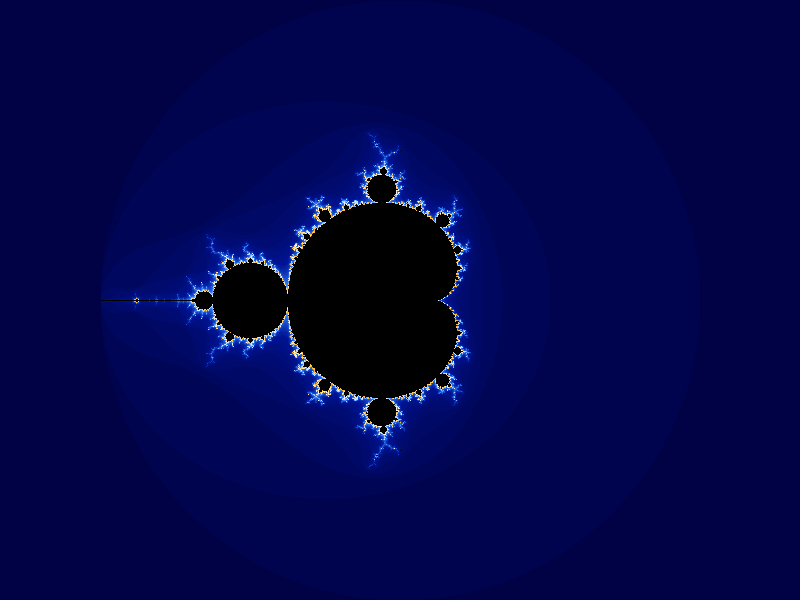
\includegraphics[width=0.55\textwidth]{img/mandelbrot.png}
    \caption{Zbiór Mandelbrota obliczony przez program w puli wątków ($800 \times 600$, \texttt{MAX\_ITER = 570})}
\end{figure}

\subsection{Opis rozwiązania}
Implementacja jest w języku \texttt{Java}. Zwracamy uwagę na kilka elementów:
\begin{itemize}
    \item \textbf{Zadanie to fragment obrazu.} Obraz dzielimy na prostokąty (domyślnie jeden wiersz
          na zadanie, 600 zadań), a każdy prostokąt jest \texttt{Callable}. Rozmiar zadania jest
          parametrem, który badamy osobno.
    \item \textbf{Brak synchronizacji na obrazie.} Wynik to tablica \texttt{int[]} z liczbą pozostałych
          iteracji każdego piksela, zamiast \texttt{BufferedImage.setRGB} z oryginału.
          Zadania zapisują rozłączne fragmenty, a \texttt{Future.get()} zapewnia widoczność
          zapisów w wątku, który odbiera wynik.
    \item \textbf{Zmienne lokalne.} W oryginale \texttt{zx, zy, cX, cY, tmp} są polami obiektu,
          więc równoległe wykonanie tego kodu miałoby wyścig. U nas są zmiennymi lokalnymi metody.
    \item \textbf{Poprawność.} Po każdym przebiegu porównujemy obraz z obrazem policzonym sekwencyjnie
          i przerywamy pomiar, gdy się różnią.
\end{itemize}
Razem ze sprawozdaniem zawarty jest pełny kod programu, program wykonujący pomiary
oraz skrypt generujący wykresy.

\section{Specyfikacja narzędzi i sprzętu}
Program został napisany w języku \texttt{Java 27} i uruchomiony na maszynie wirtualnej
\texttt{OpenJDK}, na komputerze z procesorem \texttt{Apple M4} (architektura \texttt{ARM64},
10 rdzeni: 4 wydajnościowe i 6 energooszczędnych), \texttt{16 GB} zunifikowanej pamięci
\texttt{LPDDR5} i systemem operacyjnym \texttt{macOS 26}.
Do wygenerowania wykresów użyty został \texttt{Python} z biblioteką \texttt{matplotlib}.

\subsection{Metoda pomiaru}
Mierzymy czas od utworzenia puli, przez zgłoszenie wszystkich zadań, do odebrania ostatniego
\texttt{Future} (\texttt{System.nanoTime()}). Czas obejmuje więc start wątków puli, który jest
częścią kosztu użycia danego Executora; zamknięcie puli nie jest mierzone.
Parametry: \texttt{MAX\_ITER} $\in \{500, 1000, 2000, 5000, 10000\}$, liczba wątków
$n \in \{1, 2, 4, 6, 8, 10, 12, 16\}$ dla \texttt{fixed} i \texttt{work-stealing}
(pozostałe pule nie mają tego parametru). Przed pomiarami wykonujemy pięć przebiegów
rozgrzewających JIT dla każdego Executora, a każdą konfigurację uruchamiamy trzy razy i bierzemy medianę.
Punktem odniesienia jest ten sam kod uruchomiony w jednym wątku bez Executora (\textit{sekwencyjnie}),
względem którego liczymy przyspieszenie $S = T_{seq} / T$ i efektywność $S / n$.
Dodatkowo badamy wpływ rozmiaru zadania (przy \texttt{MAX\_ITER = 2000}) oraz rozkład obciążenia
wątków: wewnątrz zadania mierzymy czas pracy, sumujemy go na wątek i liczymy indeks sprawiedliwości
Jaina $J = (\sum x)^2 / (k \sum x^2)$ oraz stosunek największego obciążenia do średniego.

\section{Algorytmy}
\begin{algorytm}[H]
\setstretch{1.4}
\begin{algorithmic}[1]
    \Procedure{compute}{$\textit{executor}, \textit{regions}$} \Comment{wątek główny}
        \State $\textit{futures} \gets$ pusta lista
        \For{\textbf{każdy} $r \in \textit{regions}$}
            \State $\textit{futures}$.\Call{add}{$\textit{executor}$.\Call{submit}{\textsc{task}($r$)}}
        \EndFor
        \For{\textbf{każdy} $f \in \textit{futures}$}
            \State $f$.\Call{get}{} \Comment{czeka na zadanie, zgłasza jego wyjątek}
        \EndFor
    \EndProcedure
    \Procedure{task}{$r$} \Comment{wątek puli}
        \For{\textbf{każdy} piksel $(x, y) \in r$}
            \State $\textit{iters}[y][x] \gets$ \Call{pixel}{$x, y$}
        \EndFor
    \EndProcedure
\end{algorithmic}
\caption{Podział na zadania i oczekiwanie na Future}
\end{algorytm}

Funkcja \textsc{pixel} jest jądrem z oryginału: dla $c = (x - 400)/150 + i\,(y - 300)/150$
iteruje $z \gets z^2 + c$ od $z = 0$, dopóki $|z|^2 < 4$ i zostały iteracje.
Koszt zadania jest bardzo nierówny: piksel należący do zbioru zużywa wszystkie \texttt{MAX\_ITER}
iteracji, a piksel daleko od zbioru kończy po kilku. Zadania leżące w środku obrazu są
więc wielokrotnie droższe od brzegowych, co wpływa na wybór rozmiaru zadania i rodzaju puli.

\paragraph{Rozkład zadań.} W \texttt{fixed} wszystkie wątki biorą zadania z jednej wspólnej kolejki,
więc wątek, który skończył, od razu pobiera następne zadanie. W \texttt{work-stealing} zadania
zgłaszane z wątku spoza puli trafiają do kolejek zgłoszeń, z których pobierają je wątki puli,
a bezczynny wątek podkrada zadania z kolejek innych. W obu przypadkach, jeśli zadań jest
dużo więcej niż wątków, obciążenie wyrównuje się samo. Gdy zadań jest tyle co wątków, żadna pula
nie może przenieść już rozpoczętego zadania na inny wątek.

\section{Implementacja}
Poniżej znajdują się najważniejsze fragmenty. Pełny kod (w tym program pomiarowy \textbf{Main}
i rysowanie obrazu) jest w katalogu \texttt{src} dołączonym do sprawozdania.

\begin{lstlisting}[caption={Klasa \textbf{Mandelbrot}: jądro obliczeń, fragmenty obrazu i podział na zadania (\texttt{src/Mandelbrot.java})}]

/**
 * Mandelbrot set on a 800x600 grid (same parameters as the Rosetta Code Java version).
 * The image is an int[] of "remaining iterations" per pixel; tasks write disjoint regions,
 * and Future.get() gives the happens-before edge back to the caller.
 */
class Mandelbrot {
    static final int WIDTH = 800, HEIGHT = 600;
    static final double ZOOM = 150;

    /** Rectangular part of the image computed by one task: [x0,x1) x [y0,y1). */
    record Region(int x0, int x1, int y0, int y1) {}

    final int maxIter;
    final int[] iters = new int[WIDTH * HEIGHT];

    Mandelbrot(int maxIter) {
        this.maxIter = maxIter;
    }

    /** Original pixel kernel: returns the number of iterations left when |z| >= 2 (0 inside the set). */
    int pixel(int x, int y) {
        double zx = 0, zy = 0, tmp;
        double cX = (x - 400) / ZOOM;
        double cY = (y - 300) / ZOOM;
        int iter = maxIter;
        while (zx * zx + zy * zy < 4 && iter > 0) {
            tmp = zx * zx - zy * zy + cX;
            zy = 2.0 * zx * zy + cY;
            zx = tmp;
            iter--;
        }
        return iter;
    }

    void compute(Region r) {
        for (int y = r.y0(); y < r.y1(); y++) {
            for (int x = r.x0(); x < r.x1(); x++) {
                iters[y * WIDTH + x] = pixel(x, y);
            }
        }
    }

    /** Reference: whole image in the calling thread, no executor. */
    void computeSequential() {
        compute(new Region(0, WIDTH, 0, HEIGHT));
    }

    /**
     * Splits the image into tasks. shape: "rows:K" (K image rows per task), "tile:K" (KxK tiles),
     * "perthread" (one block of rows per pool thread, n threads).
     */
    static List<Region> regions(String shape, int n) {
        List<Region> list = new ArrayList<>();
        if (shape.startsWith("tile:")) {
            int k = Integer.parseInt(shape.substring(5));
            for (int y = 0; y < HEIGHT; y += k)
                for (int x = 0; x < WIDTH; x += k)
                    list.add(new Region(x, Math.min(x + k, WIDTH), y, Math.min(y + k, HEIGHT)));
        } else {
            int k = shape.equals("perthread") ? (HEIGHT + n - 1) / n : Integer.parseInt(shape.substring(5));
            for (int y = 0; y < HEIGHT; y += k)
                list.add(new Region(0, WIDTH, y, Math.min(y + k, HEIGHT)));
        }
        return list;
    }
\end{lstlisting}

\begin{lstlisting}[caption={Metoda \texttt{compute} klasy \textbf{Mandelbrot}: zgłoszenie zadań do Executora i oczekiwanie na Future (\texttt{src/Mandelbrot.java})}]
    /** Submits one Callable per region and waits for all Futures; any task failure is rethrown. */
    void compute(ExecutorService executor, List<Region> regions) throws InterruptedException {
        List<Future<Void>> futures = new ArrayList<>(regions.size());
        for (Region r : regions) {
            Callable<Void> task = () -> {
                compute(r);
                return null;
            };
            futures.add(executor.submit(task));
        }
        for (Future<Void> f : futures) {
            try {
                f.get();
            } catch (ExecutionException e) {
                throw new RuntimeException("task failed", e.getCause());
            }
        }
    }
\end{lstlisting}

\begin{lstlisting}[caption={Fabryka puli (\texttt{src/Executors2.java})}]
    static ExecutorService create(String name, int n) {
        return switch (name) {
            case "single" -> Executors.newSingleThreadExecutor();
            case "fixed" -> Executors.newFixedThreadPool(n);
            case "cached" -> Executors.newCachedThreadPool();
            case "workstealing" -> Executors.newWorkStealingPool(n);
            case "virtual" -> Executors.newVirtualThreadPerTaskExecutor();
            default -> throw new IllegalArgumentException(name);
        };
    }
\end{lstlisting}


\section{Wyniki}
Sekwencyjne obliczenie obrazu trwa \num{33.6} ms dla \texttt{MAX\_ITER = 500} i \num{659.2} ms dla \texttt{MAX\_ITER = 10000}.
Czas rośnie liniowo z \texttt{MAX\_ITER}, więc ten parametr skaluje koszt obliczeń bez zmiany struktury zadań.

\subsection{Rodzaj Executora i liczba wątków}
\textbf{Rysunek~\ref{fig:times}} pokazuje czas obliczeń. Linie ciągłe to pule z parametrem $n$,
linie przerywane -- pule bez parametru, linia kropkowana -- wersja sekwencyjna.

\begin{figure}[H]
    \centering
    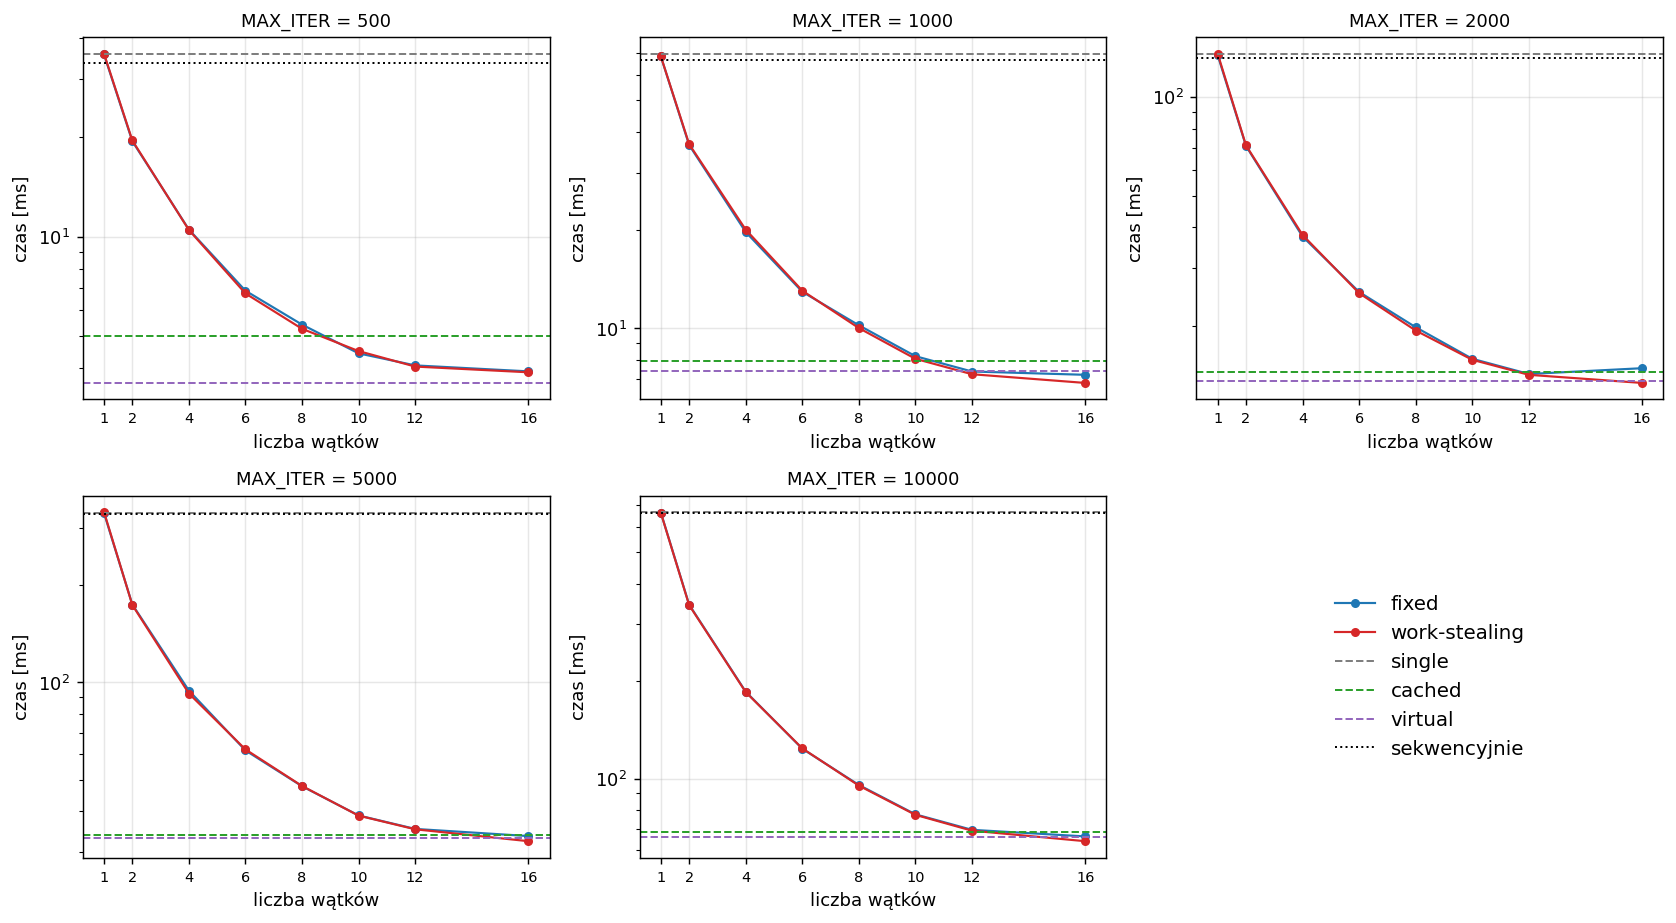
\includegraphics[width=\textwidth]{img/times.png}
    \caption{Czas obliczeń w zależności od liczby wątków (zadanie = 1 wiersz, skala logarytmiczna)}
    \label{fig:times}
\end{figure}

\textbf{Pule z jednym wątkiem} (\texttt{single}, \texttt{fixed} i \texttt{work-stealing} z $n = 1$)
są równie szybkie jak kod bez Executora, a narzut zgłaszania 600 zadań jest niewielki:
\num{35.7} ms wobec \num{33.6} ms dla \texttt{MAX\_ITER = 500} (przyspieszenie \num{0.94}) i
\num{665.7} ms wobec \num{659.2} ms dla \texttt{MAX\_ITER = 10000}. \texttt{single} i \texttt{fixed(1)} mają praktycznie ten sam czas
(\num{665.7} ms i \num{662.8} ms dla \texttt{MAX\_ITER = 10000}).

\textbf{Skalowanie.} \texttt{fixed} i \texttt{work-stealing} skalują się do 10 wątków, czyli liczby rdzeni, ale
z efektywnością mniejszą niż 1.
Przyspieszenie dla $n = 4$ wynosi \num{3.20}--\num{3.55} (efektywność \num{0.80}--\num{0.89}),
dla $n = 10$ \num{7.57}--\num{8.50}, a dla $n = 16$ \num{8.59}--\num{9.94}
(\textbf{Rysunek~\ref{fig:speedup}}). Przyspieszenie mniejsze niż $n$ nie wynika z nierównego podziału pracy (dla 10 wątków i zadań po jednym wierszu
indeks Jaina wynosi \num{1.00}, patrz niżej). Prawdopodobne przyczyny to spadek taktu procesora przy obciążeniu wielu rdzeni
oraz inne procesy w systemie -- tego nie sprawdzaliśmy.
Powyżej 10 wątków zysk jest już mały: z $n = 10$ do $n = 16$ czas dla \texttt{MAX\_ITER = 10000}
spada z \num{77.6} ms do \num{66.3} ms (\texttt{fixed}), a efektywność spada do \num{0.54}--\num{0.62}.
Dla małego \texttt{MAX\_ITER} przyspieszenie jest gorsze (\num{7.57} dla 500 i $n = 10$ wobec \num{8.50} dla 10000),
ponieważ stały koszt startu puli i zgłoszenia zadań (dla \texttt{fixed(1)} \num{2.0} ms więcej niż sekwencyjnie przy \texttt{MAX\_ITER = 500}) stanowi większą część krótkiego obliczenia.

\begin{figure}[H]
    \centering
    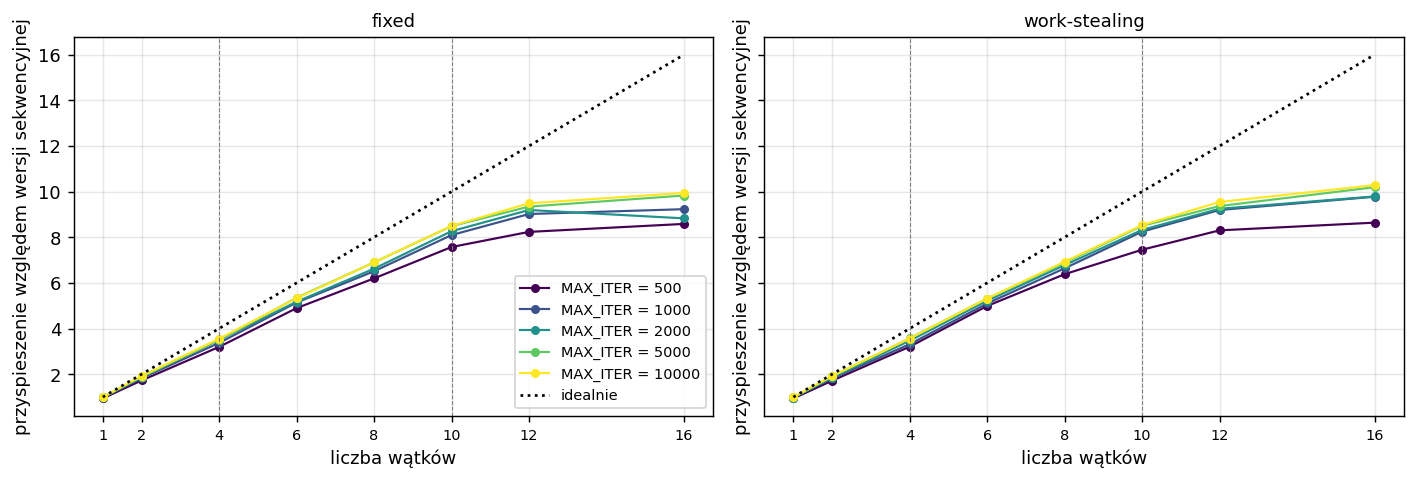
\includegraphics[width=0.85\textwidth]{img/speedup.png}
    \caption{Przyspieszenie względem wersji sekwencyjnej (zadanie = 1 wiersz); linie przerywane: 4 i 10 wątków}
    \label{fig:speedup}
\end{figure}

\textbf{\texttt{fixed} i \texttt{work-stealing}} dają prawie ten sam czas: dla $n \le 12$ różnica nie
przekracza \num{3}\%. Dopiero dla $n = 16$ \texttt{work-stealing} jest
szybszy o \num{1}--\num{10}\% (np. \num{64.1} ms wobec \num{66.3} ms dla \texttt{MAX\_ITER = 10000}).
Nie widać więc przewagi wynikającej z podkradania zadań: wszystkie zadania zgłasza jeden wątek,
a zadań jest 600, więc wspólna kolejka \texttt{fixed} nie jest wąskim gardłem.

\textbf{\texttt{cached}} tworzy wątek na każde zadanie, na które nie ma wolnego wątku. Ponieważ
zadania są zgłaszane szybciej, niż się wykonują, pula urosła do \num{30}--\num{37} wątków
(liczba rośnie z \texttt{MAX\_ITER}), czyli do kilku razy więcej niż rdzeni. Dla \texttt{MAX\_ITER} $\ge 1000$ osiąga
przyspieszenie \num{8.40}--\num{9.65}, bliskie \texttt{fixed} z 16 wątkami (\num{9.23}--\num{9.94}), ale dla
\texttt{MAX\_ITER = 500} jest wyraźnie wolniejsza (\num{5.0} ms wobec \num{3.9} ms), bo
tworzenie wielu wątków kosztuje tyle, co duża część obliczenia. Nie ma też żadnego ograniczenia
zasobów: przy dłuższych zadaniach i większej liczbie zgłoszeń liczba wątków mogłaby sięgnąć liczby zadań.

\textbf{Wątki wirtualne} są najszybsze dla krótkich obliczeń (\num{3.6} ms dla \texttt{MAX\_ITER = 500}, przyspieszenie
\num{9.31}) i dla \texttt{MAX\_ITER = 10000} osiągają przyspieszenie \num{10.00}. Zadanie jest czysto
obliczeniowe, więc wątki wirtualne nie dają tu żadnej przewagi nad pulą z $n$ równym liczbie rdzeni
poza tym, że start wątku wirtualnego jest tani; ich zaletą są zadania, które często czekają na wejście-wyjście.

\textbf{Tabela~\ref{tab:summary}} zestawia czasy i przyspieszenia.

\begin{table}[H]
    \centering
    \renewcommand{\arraystretch}{1.3}
    \begin{tabular}{|l|r|r|r|r|r|}
        \hline
        Executor & \texttt{500} & \texttt{1000} & \texttt{2000} & \texttt{5000} & \texttt{10000} \\ \hline
        sekwencyjnie & \num{33.6} / \num{1.00} & \num{66.6} / \num{1.00} & \num{131.6} / \num{1.00} & \num{330.0} / \num{1.00} & \num{659.2} / \num{1.00} \\
        \texttt{single} & \num{35.7} / \num{0.94} & \num{69.5} / \num{0.96} & \num{135.0} / \num{0.97} & \num{333.4} / \num{0.99} & \num{665.7} / \num{0.99} \\
        \texttt{fixed}, $n = 10$ & \num{4.4} / \num{7.57} & \num{8.2} / \num{8.10} & \num{15.9} / \num{8.27} & \num{38.9} / \num{8.49} & \num{77.6} / \num{8.50} \\
        \texttt{fixed}, $n = 16$ & \num{3.9} / \num{8.59} & \num{7.2} / \num{9.23} & \num{14.9} / \num{8.83} & \num{33.6} / \num{9.83} & \num{66.3} / \num{9.94} \\
        \texttt{work-stealing}, $n = 10$ & \num{4.5} / \num{7.45} & \num{8.1} / \num{8.25} & \num{15.8} / \num{8.32} & \num{38.8} / \num{8.50} & \num{77.3} / \num{8.53} \\
        \texttt{work-stealing}, $n = 16$ & \num{3.9} / \num{8.64} & \num{6.8} / \num{9.78} & \num{13.4} / \num{9.79} & \num{32.4} / \num{10.19} & \num{64.1} / \num{10.29} \\
        \texttt{cached} & \num{5.0} / \num{6.72} & \num{7.9} / \num{8.40} & \num{14.5} / \num{9.09} & \num{33.9} / \num{9.75} & \num{68.3} / \num{9.65} \\
        \texttt{virtual} & \num{3.6} / \num{9.31} & \num{7.4} / \num{9.02} & \num{13.6} / \num{9.64} & \num{33.1} / \num{9.98} & \num{65.9} / \num{10.00} \\
        \hline
    \end{tabular}
    \caption{Czas [ms] / przyspieszenie względem wersji sekwencyjnej dla kolejnych wartości \texttt{MAX\_ITER} (zadanie = 1 wiersz)}
    \label{tab:summary}
\end{table}

\subsection{Rozmiar zadania}
\textbf{Rysunek~\ref{fig:gran}} pokazuje czas dla \texttt{MAX\_ITER = 2000} przy różnym podziale obrazu:
od 600 wierszy po jeden blok wierszy na wątek (10 zadań dla $n = 10$ i 4 zadania dla $n = 4$).

\begin{figure}[H]
    \centering
    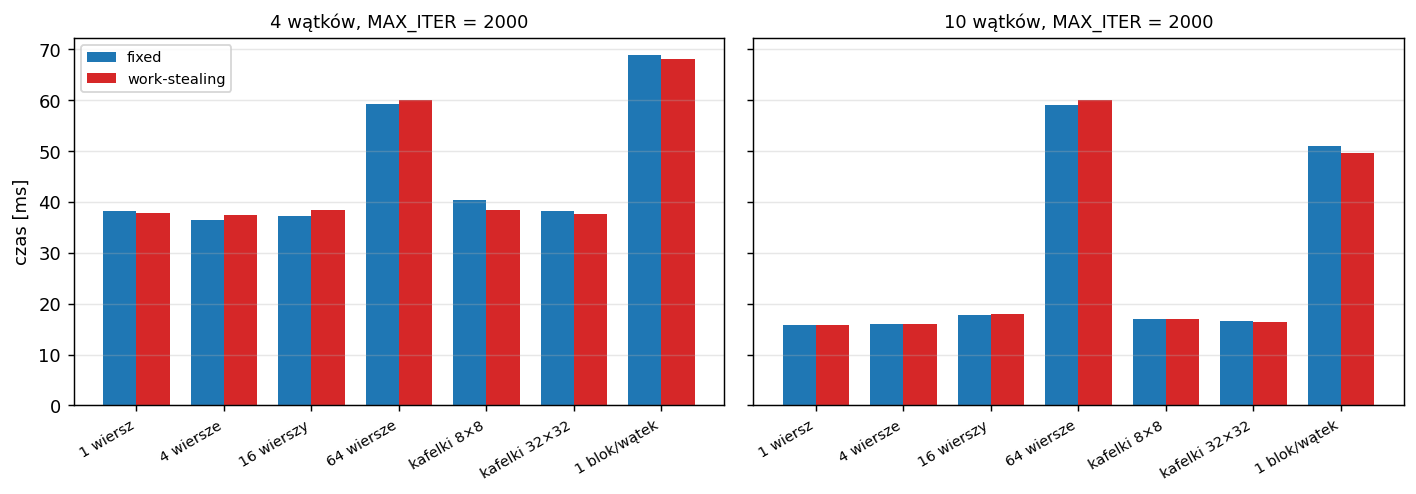
\includegraphics[width=0.85\textwidth]{img/granularity.png}
    \caption{Czas obliczeń w zależności od rozmiaru zadania, \texttt{MAX\_ITER = 2000}}
    \label{fig:gran}
\end{figure}

Dla zadań od jednego do 16 wierszy oraz kafelków czas jest niemal stały: dla $n = 10$ wynosi
\num{15.9} ms (1 wiersz), \num{17.9} ms (16 wierszy) i \num{16.6} ms (kafelki $32 \times 32$).
Bardzo małe zadania mają mały koszt: 7500 kafelków $8 \times 8$ daje \num{17.1} ms, czyli około
\num{8}\% więcej niż 600 wierszy, a to jest koszt zgłoszenia i pobrania zadań. Zbyt duże zadania są
znacznie gorsze: przy 10 zadaniach (\textit{64 wiersze}) czas rośnie do \num{59.0} ms, a przy
jednym bloku na wątek do \num{50.9} ms, czyli \num{3.21} razy więcej niż przy wierszach.
Dla $n = 4$ ten sam blok (150 wierszy) daje \num{68.8} ms wobec \num{38.3} ms dla wierszy.
Obie pule zachowują się tu tak samo (różnice do \num{5}\%).

\begin{figure}[H]
    \centering
    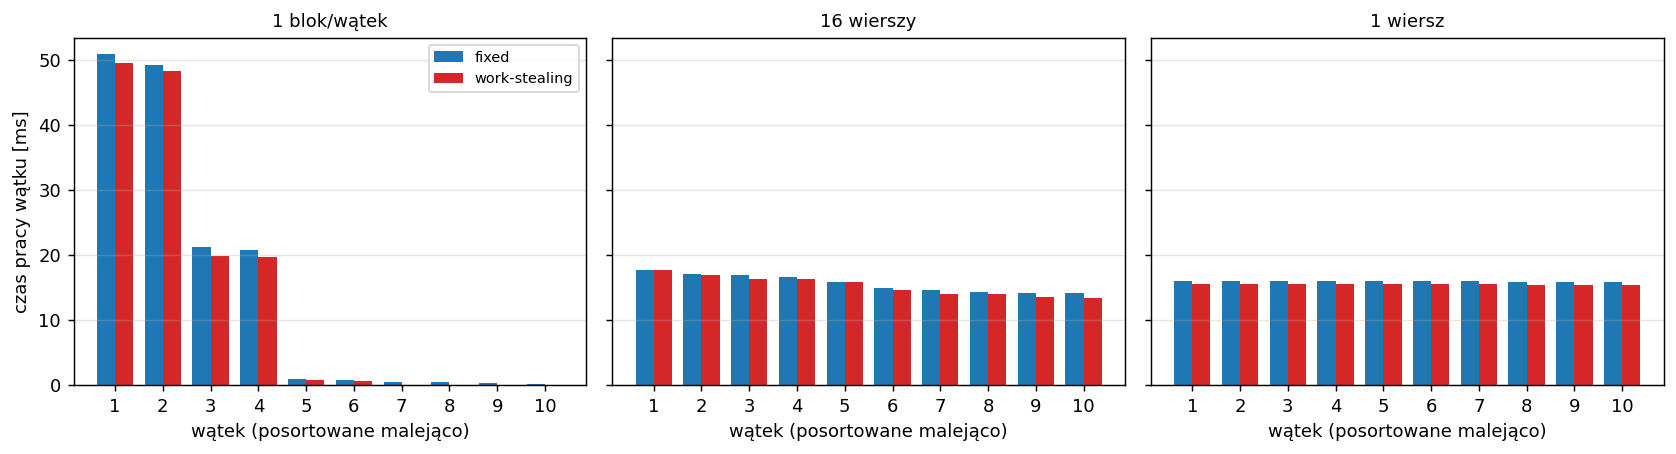
\includegraphics[width=\textwidth]{img/load.png}
    \caption{Czas pracy każdego z 10 wątków, \texttt{MAX\_ITER = 2000} (posortowany malejąco)}
    \label{fig:load}
\end{figure}

Powód widać na \textbf{Rysunku~\ref{fig:load}}. Gdy zadań jest tyle co wątków, wątek, który dostał blok
ze środka obrazu, pracuje \num{3.57} razy dłużej niż średnia, a indeks Jaina wynosi tylko \num{0.35}
(\texttt{fixed}) i \num{0.35} (\texttt{work-stealing}); pozostałe wątki są bezczynne, a czas całości
(\num{51.7} ms) wyznacza najbardziej obciążony wątek. Podkradanie nie pomaga, bo jedyne zadanie
każdego wątku jest już wykonywane i nie można go podzielić. Dla zadań po 16 wierszy indeks $J$ wynosi \num{0.99},
a stosunek maksimum do średniej \num{1.16}, a dla pojedynczych wierszy $J = $ \num{1.00}
(czas całości \num{18.0} ms i \num{16.0} ms).

\section{Weryfikacja poprawności}
Wynik obliczenia jest deterministyczny: wartość piksela zależy tylko od jego współrzędnych i \texttt{MAX\_ITER}.
Dlatego poprawność obliczeń w puli sprawdzamy, porównując cały obraz z obrazem policzonym sekwencyjnie w jednym wątku.
Sprawdzamy to na cztery sposoby.
\begin{enumerate}
    \item \textbf{Każdy pomiar sprawdza swój wynik.} Po każdym przebiegu (poza mierzonym czasem) \texttt{Main}
          porównuje tablicę \texttt{iters} z referencją przez \texttt{Arrays.equals}. Niezgodność rzuca \texttt{AssertionError}.
          Wyjątek rzucony w zadaniu jest przekazywany przez \texttt{Future.get()} i zgłaszany dalej,
          a domyślny handler wyjątków kończy program z błędem. Pula musi się też zamknąć w 10 s
          (\texttt{awaitTermination}). Wszystkie \num{402} przebiegi pomiarowe (wyniki w tabelach i na wykresach)
          przeszły to sprawdzenie, a \texttt{make bench} zakończył się bez błędu.
    \item \textbf{Test wszystkich pul i podziałów.} Program \texttt{Verify} (\texttt{make verify}) uruchamia każdy z 5 Executorów dla
          wszystkich 6 podziałów obrazu (1, 7 i 64 wiersze, kafelki $8 \times 8$ i $50 \times 50$, jeden blok na wątek)
          i liczby wątków $n \in \{1, 3, 7, 16\}$ (dla pul z parametrem), po 3 razy: razem \num{198} przebiegów.
          Wszystkie dały obraz identyczny z referencją. Część rozmiarów nie dzieli 600 ani 800 (np. 7 i 64 wiersze), więc sprawdzane są
          też zadania o różnych rozmiarach, w tym ostatnie, niepełne.
    \item \textbf{Poprawność jądra.} Referencja też mogłaby być błędna, więc sprawdzamy ją niezależnie od równoległości.
          Pole zbioru wynosi $\approx 1{,}5066$, a z obrazu (liczba pikseli należących do zbioru razy pole piksela $1/150^2$)
          dostajemy \num{1.5164} dla \texttt{MAX\_ITER = 570} i \num{1.5104} dla \texttt{MAX\_ITER = 5000}.
          Wartość zbliża się do prawdziwej od góry wraz ze wzrostem \texttt{MAX\_ITER}, jak powinna, bo przy małym \texttt{MAX\_ITER}
          część punktów leżących tuż poza zbiorem nie zdążyła jeszcze uciec i jest zaliczana do zbioru. Punkt $c = 0$ należy do zbioru, a punkt w rogu obrazu ucieka od razu.
          Pętla z oryginału (warunek \texttt{< 4}) uznaje punkt $c = -2$ leżący na brzegu za uciekający,
          co nie wpływa na wynik, bo to jeden punkt miary zero.
    \item \textbf{Czy test wykrywa błędy?} Oryginalny kod przechowuje \texttt{zx, zy, cX, cY, tmp} w polach obiektu.
          Wersja z tymi polami współdzielonymi przez wątki (klasa \texttt{RacyMandelbrot} w \texttt{Verify}, pula \texttt{fixed}, $n = 8$)
          dała inny obraz w \num{1} z \num{30} przebiegów, w najgorszym przypadku w \num{5261} pikselach.
          Test wykrywa więc wyścig, ale wyścig jest niedeterministyczny: pojedynczy poprawny przebieg go nie wyklucza.
\end{enumerate}
Brak wyścigu w naszym kodzie wynika więc z konstrukcji, a nie tylko z testów: każdy piksel liczą
zmienne lokalne metody, zadania zapisują rozłączne fragmenty tablicy, a \texttt{Future.get()} zapewnia
widoczność tych zapisów w wątku głównym (zależność \textit{happens-before}). Nie używaliśmy narzędzi do wykrywania
wyścigów (np. ThreadSanitizer), a test porównuje tylko wynik końcowy.

\section{Wnioski}
Najważniejszy dla wydajności jest podział na zadania, a nie wybór między \texttt{fixed} a \texttt{work-stealing}.
Koszt wierszy obrazu jest bardzo nierówny, więc zadania muszą być dużo liczniejsze niż wątki:
wtedy każda pula wyrównuje obciążenie sama (Jain $\approx 1$) i osiąga przyspieszenie do \num{8.50} na 10 rdzeniach
(\num{9.94} dla 16 wątków). Zadań nie warto robić mniejszych niż kilka wierszy, bo rośnie narzut
(+\num{8}\% dla kafelków $8 \times 8$), a podział „jedno zadanie na wątek” traci do \num{3.21} razy
na czasie, nawet gdy pula ma tyle wątków co rdzeni.

Liczba wątków w \texttt{fixed} powinna być zbliżona do liczby rdzeni: powyżej 10 wątków efektywność spada
do \num{0.54}--\num{0.62}, a zysk czasu jest niewielki. \texttt{work-stealing} jest tak samo
szybki jak \texttt{fixed} i sam dobiera równoległość, więc jest wygodnym wyborem domyślnym dla zadań obliczeniowych.
\texttt{single} służy tylko do wykonywania zadań po kolei, a nie do przyspieszania. \texttt{cached} wypada dobrze dla
dużych \texttt{MAX\_ITER}, ale tworzy dziesiątki wątków i nie ma ograniczenia ich liczby, więc przy zadaniach
obliczeniowych jest ryzykowna. Wątki wirtualne dają podobny czas jak pula dopasowana do rdzeni
i upraszczają kod, jednak ich zaletą są zadania blokujące, a nie obliczeniowe.

\begin{thebibliography}{9}
    \bibitem{rosetta} Rosetta Code: \textit{Mandelbrot set -- Java}. \url{http://rosettacode.org/wiki/Mandelbrot_set\#Java}
    \bibitem{tutorial} Oracle: \textit{Executors}. \url{https://docs.oracle.com/javase/tutorial/essential/concurrency/executors.html}
    \bibitem{executors} \url{http://docs.oracle.com/javase/8/docs/api/java/util/concurrent/Executors.html}
    \bibitem{future} \url{http://docs.oracle.com/javase/8/docs/api/java/util/concurrent/Future.html}
    \bibitem{agh} \url{https://home.agh.edu.pl/~funika/tw/lab8/}
\end{thebibliography}

\end{document}
